Um in die Einstellungen für die Monitore zu gelangen, klicken Sie im \enquote{Data-Input-Menü} auf den Punkt \enquote{Monitore verwalten} (siehe \autoref{fig:instr_admin_monitors_dimenu}).\\
\\
\begin{figure}[H]
\centering
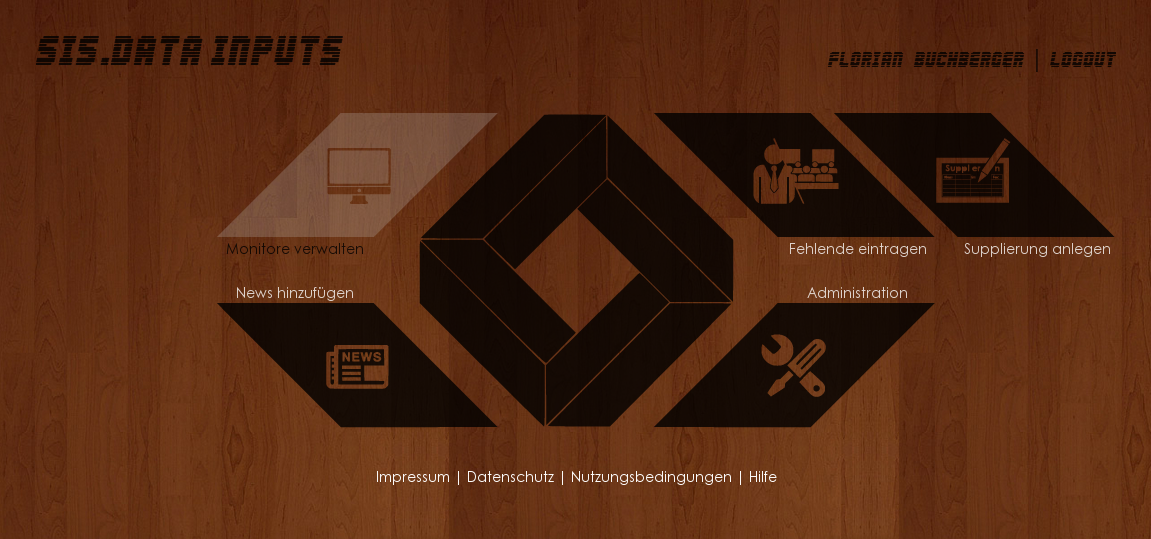
\includegraphics[keepaspectratio=true, width=14cm]{images/screenshots/data-inputs.png}
\caption{Data-Input-Menü}
\label{fig:instr_admin_monitors_dimenu}
\end{figure}
Nach dem Öffnen der Seite werden oben im Fenster die aktiven Monitore aufgelistet. Darunter sind die Einstellungen zu finden.\\
\\
\begin{figure}[H]
\centering
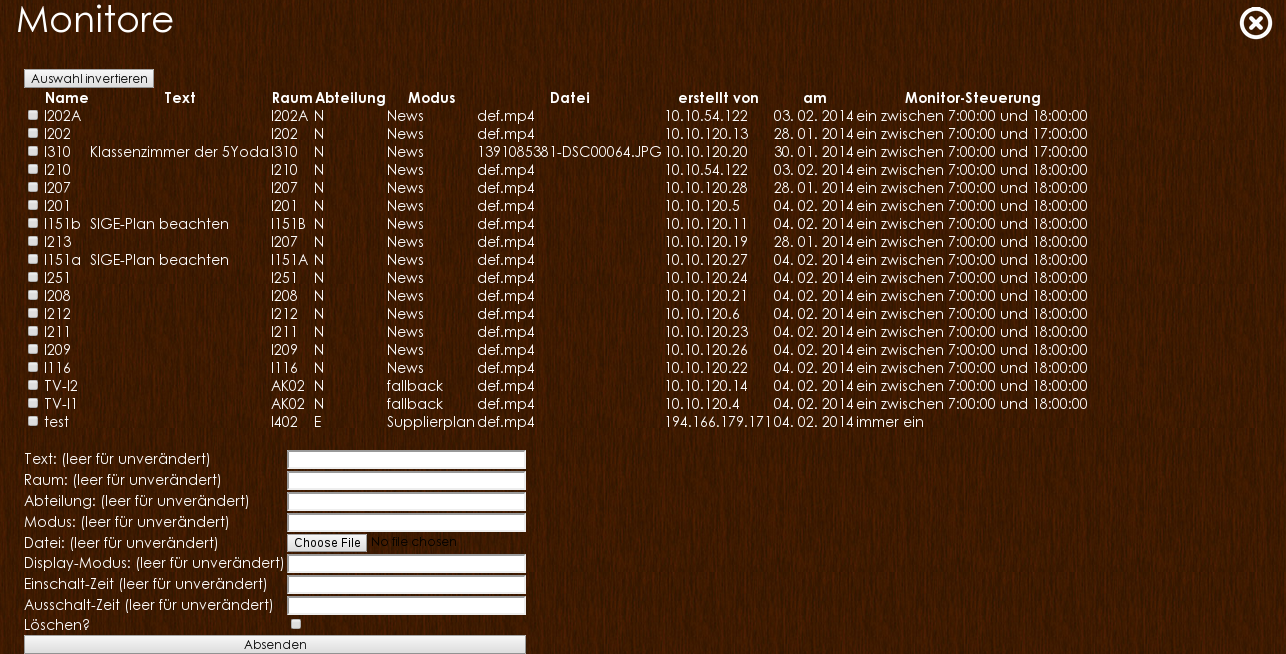
\includegraphics[keepaspectratio=true, width=14cm]{images/screenshots/monitors.png}
\caption{Monitor-Einstellungen}
\label{fig:instr_admin_monitors_site}
\end{figure}
Die Monitore, deren Einstellungen verändert werden sollen, müssen mit einem Klick auf die Checkbox links neben der Anzeige ausgwählt werden. Es können mehrere ausgewählt werden. Mit dem Button \enquote{Auswahl invertieren} werden alle gesetzten Checkbox rückgesetzt, und umgekehrt.
\\
\subsection{Hinzufügen}

Für folgendes wird vorausgesetzt, dass das von uns zur Verfügung gestellte Image verwendet wird. Dieses kann unter folgender Adresse runtergeladen werden:\\ \href{https://sis.htlinn.ac.at/sis.img}{https://sis.htlinn.ac.at/sis.img}\\
Das Image ist 4 GB groß, wir empfehlen deshalb, das Image ohne Proxy-Einstellung mit der Adresse \href{http://sis.clients.htlinn.ac.at/sis.img}{http://sis.clients.htlinn.ac.at/sis.img} im Schulnetz zu laden. Das Image sollte auf eine SD-Karte mit mindestens 3965190144 Bytes Speicherplatz gespielt werden (Getestet wurde mit \enquote{SanDisk Extreme 4GB}).\\
Der vordefinierte Benutzer hat die Kennung \enquote{pi} und das Passwort \enquote{sis}.\\
\\
Ein neuer Monitor kann nicht über das Web-Interface hinzugefügt werden, die Monitore registrieren sich selbstständig am Server. Nach der Registrierung stehen sie zur Verwaltung zur Verfügung.\\
Damit sich die Monitore registrieren können, müssen sie ihre eigene Identität kennen. Diese wird in der Datei /etc/sis.conf definiert.\\

\begin{lstlisting}[style=custom,  caption={Beispiel /etc/sis.conf},label={lst:instr_admin_sisconf}]
name=test-monitor
\end{lstlisting}
Die Form des Namenseintrags ist im Beispiel  \autoref{lst:instr_admin_sisconf} ersichtlich.\\
Wenn der Name des Monitors geändert wird, sollte aus Gründen der Übersichtlichkeit und Nachvollziehbarkeit darauf geachtet werden, dass der Hostname des Raspberry Pis mit dem Namen übereinstimmt. Dazu wird die Datei /etc/hostname bearbeitet. Damit der Host nicht neu gestartet werden muss, kann mit dem Befehl \enquote{hostname} der Hostname zusätzlich auch direkt geändert werden. \\
\textit{Beispiel}: hostname I386\\
\\
\textit{Achtung:} Da es zu Problemen mit manchen Programmen (wie zum Beispiel \textit{sudo}) kommen kann, sollte in er Datei /etc/hosts ein Eintrag für den Hostnamen angelegt werden, welcher auf die lokale Adresse zeigt (üblicherweise die Loopback-Adresse 127.0.1.1).\\
\\
\textit{Achtung:} Die Software lässt es zu, dass mehrere Monitore den selben Namen tragen. Dies sollte allerdings vermieden werden.

\subsection{Entfernen}

Um einen Monitor aus der Liste der aktiven Monitore zu entfernen, wählen Sie den jeweiligen Monitor über die Checkbox aus, setzen Sie die \enquote{Löschen?}-Checkbox und klicken Sie auf \enquote{Änderungen anwenden}.\\
\\
\textit{Achtung:} Sollte der Monitor nach dem Entfernen noch eingeschalten sein, so wird sich dieser, sofern die Standard-Konfiguration eingestellt ist, wieder neu registrieren.

\subsection{Text verändern}

Der Text, der am linken unterem Eck des Monitors kann über das Eingabefeld \enquote{Text} geändert werden. Wird das Feld leer gelassen, so wird der alte Wert beibehalten.\\
\\
\textit{Achtung:} Leerzeichen werden nicht als leer erkannt.

\subsection{Raum verändern}

Für die Darstellung des Stundenplanes des jeweiligen Raumes wird jedem Monitor ein Raum zugeordnet. Diese Einstellung kann über das Eingabefeld \enquote{Raum} angepasst werden. Durch Doppelklick auf das Eingabefeld öffnet sich - sofern der verwendete Browser diese Funktion unterstützt - ein Menü, in dem durch Eingeben gesucht werden kann. Wird das Feld leer gelassen, so wird der alte Wert beibehalten.

\subsection{Abteilung verändern}

Die News können Abteilungen zugeordnet werden. Ebenso ist der Supplierplan für jede Abteilung anders. Als Folge daraus gibt es eine Einstellungsmöglichkeit für die Abteilung. Durch Doppelklick auf das Eingabefeld öffnet sich - sofern der verwendete Browser diese Funktion unterstützt - ein Menü, in dem durch Eingeben gesucht werden kann. Wird das Feld leer gelasen, so wird der alte Wert beibehalten.

\subsection{Modus verändern}

Um die ausgewählten Monitore auf Supplierplan, Stundenplan, News etc. umzuschalten, wird das Eingabefeld \enquote{Modus} verwendet. In diesem Feld sind folgende Werte zulässig:
\begin{itemize}
	\item News
	\item Stundenplan
	\item Supplierplan
	\item Supplierplan \& News
	\item Bild
	\item (Video)
	%\item (fallback)
\end{itemize}
Durch Doppelklick auf das Eingabefeld öffnet sich - sofern der verwendete Browser diese Funktion unterstützt - ein Menü mit den möglichen Werten. Wird das Feld leer gelassen, so wird der alte Wert beibehalten.\\
\\
Der Modus \enquote{Video} ist zwar implementiert, allerdings ist der Raspberry Pi nicht in der Lage, die Videos wiederzugeben.\\
%Der Modus \enquote{fallback} fährt den Monitor auf das FTKL-Schnitzel-Suppla-Projekt.\\ 
%\textit{Achtung:} Es ist nicht über das Web-Interface möglich, den Monitor wieder auf das SIS-Projekt zurückzuholen.

\subsection{Datei verändern}

Für die Modi \enquote{Bild} und \enquote{Video} muss eine Datei hochgeladen werden, welche dann angezeigt wird.\\ 
Unterstützte Dateitypen sind:
\begin{itemize}
	\item JPG, JPEG
	\item PNG
	\item GIF
	\item MP4, MPEG
\end{itemize}
Die maximale Dateigröße ist limitiert durch:
\begin{itemize}
	\item das Upload-Script auf 800 MB
	\item den Upload-HTML-Tag auf 800 MB
	\item die PHP-Konfiguration am Server (Stand: 2014-02-28) auf 128 MB
\end{itemize}
Wird das Feld leer gelassen, so wird der alte Wert beibehalten.\\

\subsection{Display-Modus verändern}

Die Raspberry Pis verfügen über einen Mechanismus, um den angeschlossenen Monitor ein- bzw auszuschalten.\\
Es sind folgende Modi möglich:
\begin{itemize}
	\item permanent Ein
	\item permanent Aus
	\item automatisch
\end{itemize}
Im automatischen Modus werden die Einstellungen von \ref{instr_admin_moni_time_on} und \ref{instr_admin_moni_time_off} verwendet.\\
\\
Wird das Feld leer gelassen, so wird der alte Wert beibehalten.\\

\subsubsection{Einschalt-Zeit}
\label{instr_admin_moni_time_on}

Bestimmt die Zeit, an dem sich der angeschlossene Monitor einschalten soll.\\
\textit{Beispiele:}
\begin{tabbing}
\hspace{2cm}\=\kill
7 \> 7 Uhr früh\\ 
6:35 \> 6:35 früh\\
17:05:11 \> 5:05:11 nachmittags
\end{tabbing}
Wird das Feld leer gelassen, so wird der alte Wert beibehalten.\\

\subsubsection{Ausschalt-Zeit}
\label{instr_admin_moni_time_off}

Analog zu \ref{instr_admin_moni_time_on}.
